Probability of  transition,p is given by
\begin{align}
    p =  \frac{1}{8} \\
    \pr{X = 0} = \frac{9}{10} \\
    \pr{X = 1} = \frac{1}{10}
\end{align}
\begin{center}
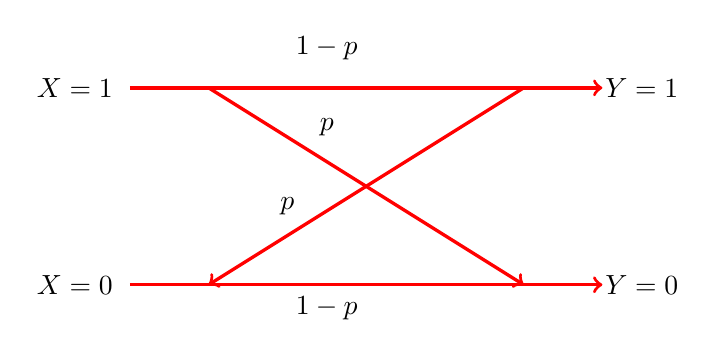
\begin{tikzpicture}
\begin{scope}[red,very thick,->]
    \draw  (0,0) -- (6,0);
   \draw (1,0) -- (5,-2.5);
   \draw (5,0) -- (1,-2.5);
   \draw (0,-2.5) -- (6,-2.5);
\end{scope}
   \node at (-0.7,0) {$\displaystyle X = 1 $};
   \node at (6.5,0)  {$\displaystyle Y = 1$};
   \node at (-0.7,-2.5) {$\displaystyle X = 0$};
   \node at (6.5,-2.5) {$\displaystyle Y = 0$};
   \node at (2.5,0.5) {$\displaystyle 1-p$};
   \node at (2.5,-2.8) {$\displaystyle 1-p$};
   \node at (2.5,-0.5) {$\displaystyle p$};
   \node at (2,-1.5) {$\displaystyle p$};
\end{tikzpicture}
\end{center}
\begin{center}
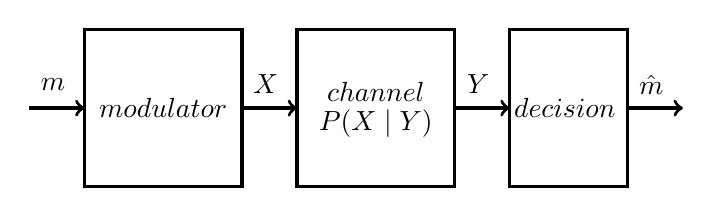
\begin{tikzpicture}
\begin{scope}[black,very thick,->]
         \draw (-0.3,0) rectangle (1.7,2); 
    \draw (2.4,0) rectangle  (4.4,2);
    \draw [->] (1.7,1) -- (2.4,1);
    \draw [->] (4.4,1) -- (5.1,1);
    \draw (5.1,0) rectangle (6.6,2);
    \draw [->] (6.6,1) -- (7.3,1);
    \draw [->] (-1,1) -- (-0.3,1);
\end{scope}
    \node at (1.5,1.5) {$\displaystyle $};
    \node at (1.5,0.5) {$\displaystyle $};
    \node at  (0.7,1)  {$\displaystyle modulator$};
    \node at  (-0.7,1.3)  {$\displaystyle m$};
    \node at  (2,1.3)  {$\displaystyle X$};
    \node at  (4.7,1.3)  {$\displaystyle Y$};
    \node at  (6.9,1.3)  {$\displaystyle \hat{m}$};
    \node at  (5.8,1)  {$\displaystyle decision$};
    \node at  (3.4,1.2)  {$\displaystyle channel$};
    \node at  (3.4,0.8)  {$\displaystyle P(X \mid Y)$};
\end{tikzpicture}
(here $m$ and $X$ can be considered similar)
\end{center}
$\therefore$ Probability of error is defined as 
\begin{align}
    P_e = \pr{\hat{m} \neq m}
\end{align}
Probability of being correct is defined as
\begin{align}
    P_c & = 1 - P_e  \\
        & = 1 - \pr{\hat{m} \neq m} \\
        & = \pr{\hat{m} = m} 
\end{align}
Optimum detector maxmize $P_c$ or equivalently minimize $P_e$ \\ Probability of making correct decision, for a given received y 
\begin{align}
    P_c & = \pr{\hat{m} = m} \\
        & = p(m_i \mid y) p(y) \\
        & = p(x_i \mid y) p(y)
\end{align}
Using Bayes theorem,
\begin{align}
    P_c & = p(y \mid x_i) p(x_i)
\end{align}
To maximize $P_c$ we use \textbf{Maximum a Posterior Detector (MAP)} rule , for a given $Y$
\begin{align}
    \hat{m} \implies m_i \ \ if \ \ \frac{p(y \mid x_i) p(x_i)}{p(y \mid x_j) p(x_j)} \geq 1
\end{align}
Now , when Y = 1 then $\hat{m}$ = 0 if
 
\begin{align}
    \frac{p(y = 1 \mid x = 0) p(x=0)}{p(y =1  \mid x = 1) p(x=1)} \geq 1 \\
\implies  \frac{p(y = 1 \mid x = 0) p(x=0)}{p(y =1  \mid x = 1) p(x=1)} \\
= \frac{\frac{1}{8} \cdot \frac{9}{10}}{\frac{7}{8} \cdot \frac{1}{10}}  \\
= \frac{9}{7} \geq 1
\end{align}
when Y = 0 then $\hat{m}$ = 0 if
\begin{align}
        \frac{p(y = 0 \mid x = 0) p(x=0)}{p(y = 0  \mid x = 1) p(x=1)} \geq 1 \\
\implies  \frac{p(y = 0 \mid x = 0) p(x=0)}{p(y = 0 \mid x = 1) p(x=1)} \\
= \frac{\frac{7}{8} \cdot \frac{9}{10}}{\frac{1}{8} \cdot \frac{1}{10}}  \\
= 63 \geq 1        
\end{align}
In both cases MAP detector suggest that message will be $\hat{m}$ = 0 \\
$\therefore$ probability of error 
\begin{multline}
    P_e  = \pr{\hat{m} \neq 0 \mid X = 0 } \pr{X = 0} \\ + \pr{\hat{m} \neq 1 \mid X = 1} \pr{X = 1} 
\end{multline}
\begin{align}    
    & = 0 + 1 \cdot \frac{1}{10} \\
    & = \frac{1}{10} 
\end{align}
So answer will be \brak{D}